\begin{figure*}[!t]
\centering
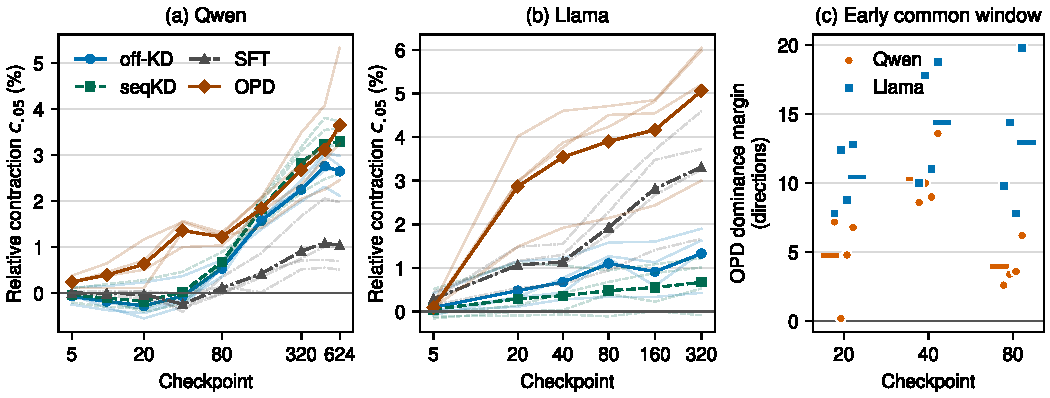
\includegraphics[width=\textwidth]{figures/fig1_main_trajectories.pdf}
\caption{纯激活、纯权重与功能轨迹。上行为 Qwen，下行为 Llama；各列依次为 activation ER、TPNT 相对 null 的 excess lift、PABS drift $10^4(1-\mathrm{PABS})$ 和 equal-5 相对功能压缩。四列量纲不同，原始纵轴幅度不可跨列比较；曲线仅连接实际 checkpoint。功能谱呈现了前三类坐标未共同复现的训练设置分离。}
\label{fig:main}
\end{figure*}

\begin{table*}[!t]
\centering
\small
\setlength{\tabcolsep}{5pt}
\begin{tabular}{lccc}
\toprule
模型 & Activation suite $A$ & Functional $C_5$ & Weight $P_{k,5}$ \\
\midrule
Llama & .556 & \textbf{.743} & .688 \\
Qwen & .595 & \textbf{.708} & .521 \\
\bottomrule
\end{tabular}
\caption{严格共同网格上的 OPD 识别（checkpoint-held-out AUC）。每个模型使用 64 个共同状态、相同 equal-5 模块和 folds。$A$ 是包含 ER、PR、top-1/8/32 share、raw/centered anisotropy 与 step-0 CKA 的八维纯激活特征组，不是图~\ref{fig:main} 中的 ER 单项。}
\label{tab:identification}
\end{table*}

\begin{table*}[!t]
\centering
\small
\setlength{\tabcolsep}{4pt}
\begin{tabular}{lrrrrr}
\toprule
模型 & $M_{\min}^{\mathrm{early}}$ & OPD NCD & SFT NCD & off-KD NCD & seqKD NCD \\
\midrule
Qwen & .200 & \textbf{50.423} & 9.554 & 31.017 & 37.793 \\
Llama & 7.800 & \textbf{77.594} & 39.683 & 17.518 & 11.093 \\
\bottomrule
\end{tabular}
\caption{共同早期排序与全轨迹压缩剂量。$M_{\min}^{\mathrm{early}}$ 是四核心域和共同早期 checkpoint 上的最小 OPD 连续边际（directions）；正值排除该范围内的排序反转。NCD 在 $\log(1+t)$ 上积分至 $T=320$（directions$\times$log-step），衡量压缩深度与持续时间。两列尺度不可直接比较。}
\label{tab:ncd}
\end{table*}

\begin{figure*}[!t]
\centering
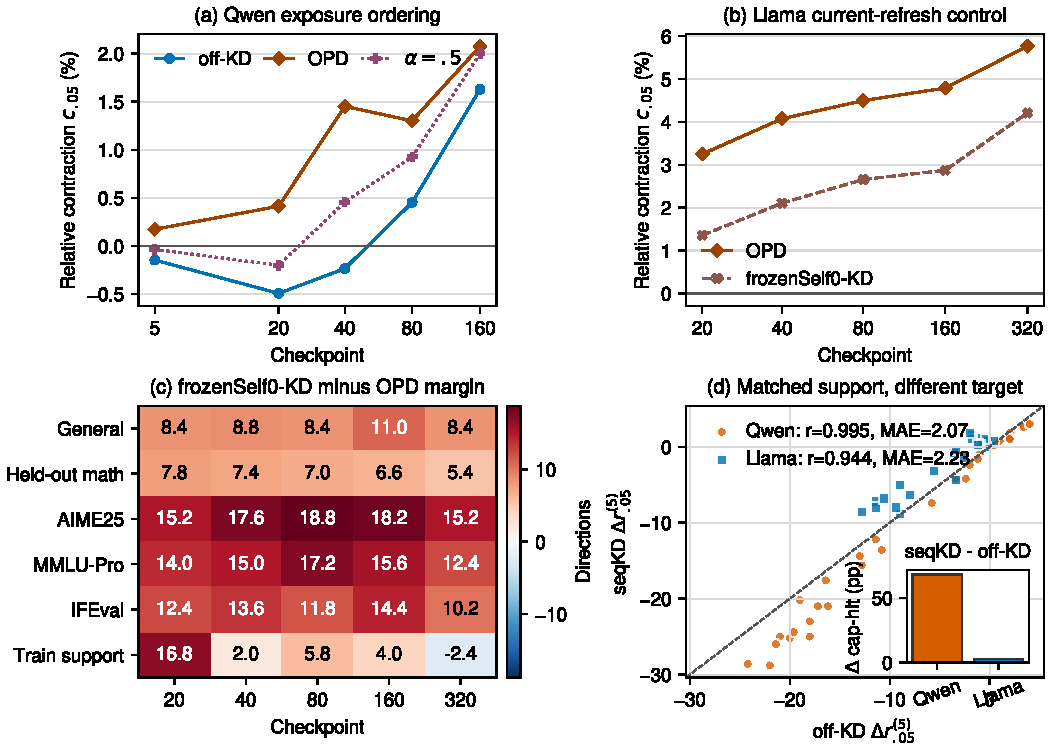
\includegraphics[width=\textwidth]{figures/fig2_support_controls.pdf}
\caption{Sequence exposure 与 refresh 对照。（a）Qwen $\alpha=.5$ 相对 off-KD 和 OPD 的有序轨迹。（b）Llama OPD 与 frozenSelf0-KD 在五个固定外部域上的等域平均绝对轨迹。（c）对应的逐域配对边际；正值表示持续刷新的 OPD 更压缩，粗黑线为外部域均值。图例中的 Math、AIME、MMLU 和 Mean 分别表示 held-out math、AIME25、MMLU-Pro 和五域均值。}
\label{fig:controls}
\end{figure*}

\begin{table*}[!t]
\centering
\small
\setlength{\tabcolsep}{2.7pt}
\textbf{A. off-KD 与 seqKD 的逐域 equal-5 路径一致性（Pearson $r$/MAE directions）}\\[2pt]
\begin{tabular}{lccccc}
\toprule
模型 & General & Math & MMLU-Pro & IFEval & Pooled \\
\midrule
Qwen & .995/1.13 & .996/2.67 & .998/2.18 & .999/2.29 & .995/2.07 \\
Llama & -.771/2.53 & .971/1.73 & .968/2.23 & .824/2.40 & .944/2.23 \\
\bottomrule
\end{tabular}

\vspace{4pt}
\textbf{B. 匹配训练设置的终点行为（\%）}\\[2pt]
\begin{tabular}{llrrrrrrr}
\toprule
模型 & 设置 & \multicolumn{2}{c}{MATH500} & \multicolumn{3}{c}{MMLU-Pro} & \multicolumn{2}{c}{IFEval} \\
\cmidrule(lr){3-4}\cmidrule(lr){5-7}\cmidrule(lr){8-9}
 & & Acc. & Cap & Strict & Flex. & Extract & Prompt & Instr. \\
\midrule
Qwen & off-KD & 79.4 & 4.8 & 35.4 & 57.1 & 47.3 & 23.1 & 36.5 \\
 & seqKD & 72.4 & 73.0 & 30.6 & 58.1 & 54.1 & 24.4 & 39.3 \\
Llama & off-KD & 8.2 & 91.8 & 14.2 & 16.4 & 50.3 & 19.6 & 33.2 \\
 & seqKD & 10.2 & 94.6 & 13.1 & 15.4 & 51.6 & 19.2 & 31.5 \\
\bottomrule
\end{tabular}
\caption{Matched-support 的功能路径与行为读出。A 使用完全匹配的非零 checkpoint；MAE 是逐 checkpoint 的方向差。B 使用 Qwen step 624 与 Llama step 320；Cap 为 generation-cap hit，Extract 为 extraction failure，Prompt/Instr. 为 IFEval prompt/instruction strict。}
\label{tab:support-readout}
\end{table*}

\begin{figure*}[!t]
\centering
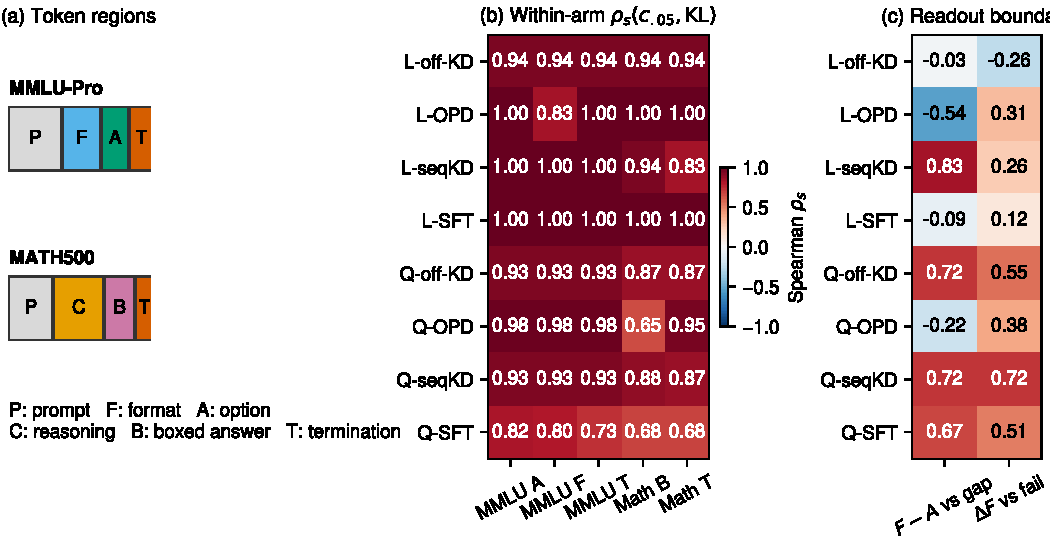
\includegraphics[width=\textwidth]{figures/fig3_regional_output.pdf}
\caption{区域输出关系。（a）每个模型和训练设置内，equal-5 功能压缩与区域 full-vocabulary KL 的跨 checkpoint Spearman。MMLU-Pro 的列为格式 $F$、正确选项标签 $A$ 和终止 $T$；MATH500 的列为推理 $C$、boxed answer $B$ 和终止 $T$。（b）MMLU-Pro 格式--答案 signed-NLL contrast 与 strict--flexible gap，以及格式 NLL 与 extraction failure 的相关。L 和 Q 分别表示 Llama 与 Qwen；每格数值给出相关系数。}
\label{fig:regional}
\end{figure*}

\begin{table*}[!t]
\centering
\small
\setlength{\tabcolsep}{4pt}
\begin{tabular}{llcc}
\toprule
模型/域 & 区域 & Held-out $R^2$: $C_5$ & Best $P_{k,5}$ \\
\midrule
Llama / MMLU-Pro & $A/F/T$ & \textbf{.869/.932/.468} & .743/.788/.459 \\
Llama / MATH500 & $B/T$ & .561/\textbf{.812} & \textbf{.615}/.647 \\
Qwen / MMLU-Pro & $A/F/T$ & \textbf{.426/.577/.596} & .243/.318/.443 \\
Qwen / MATH500 & $B/T$ & \textbf{.227}/.604 & .167/\textbf{.718} \\
\bottomrule
\end{tabular}
\caption{区域 full-vocabulary KL 的样本外预测。$C_5$ 与 $P_{k,5}$ 使用相同五模块、共同状态和 checkpoint-held-out folds。数值按区域顺序排列；粗体为逐区域更高的 $R^2$。后补 Math $C$ 的轨迹内和 checkpoint-demeaned 结果在正文报告，其 matched held-out 横向比较不在本表中。}
\label{tab:regional-prediction}
\end{table*}
